\chapter{Proverb 5}

\begin{figure}
  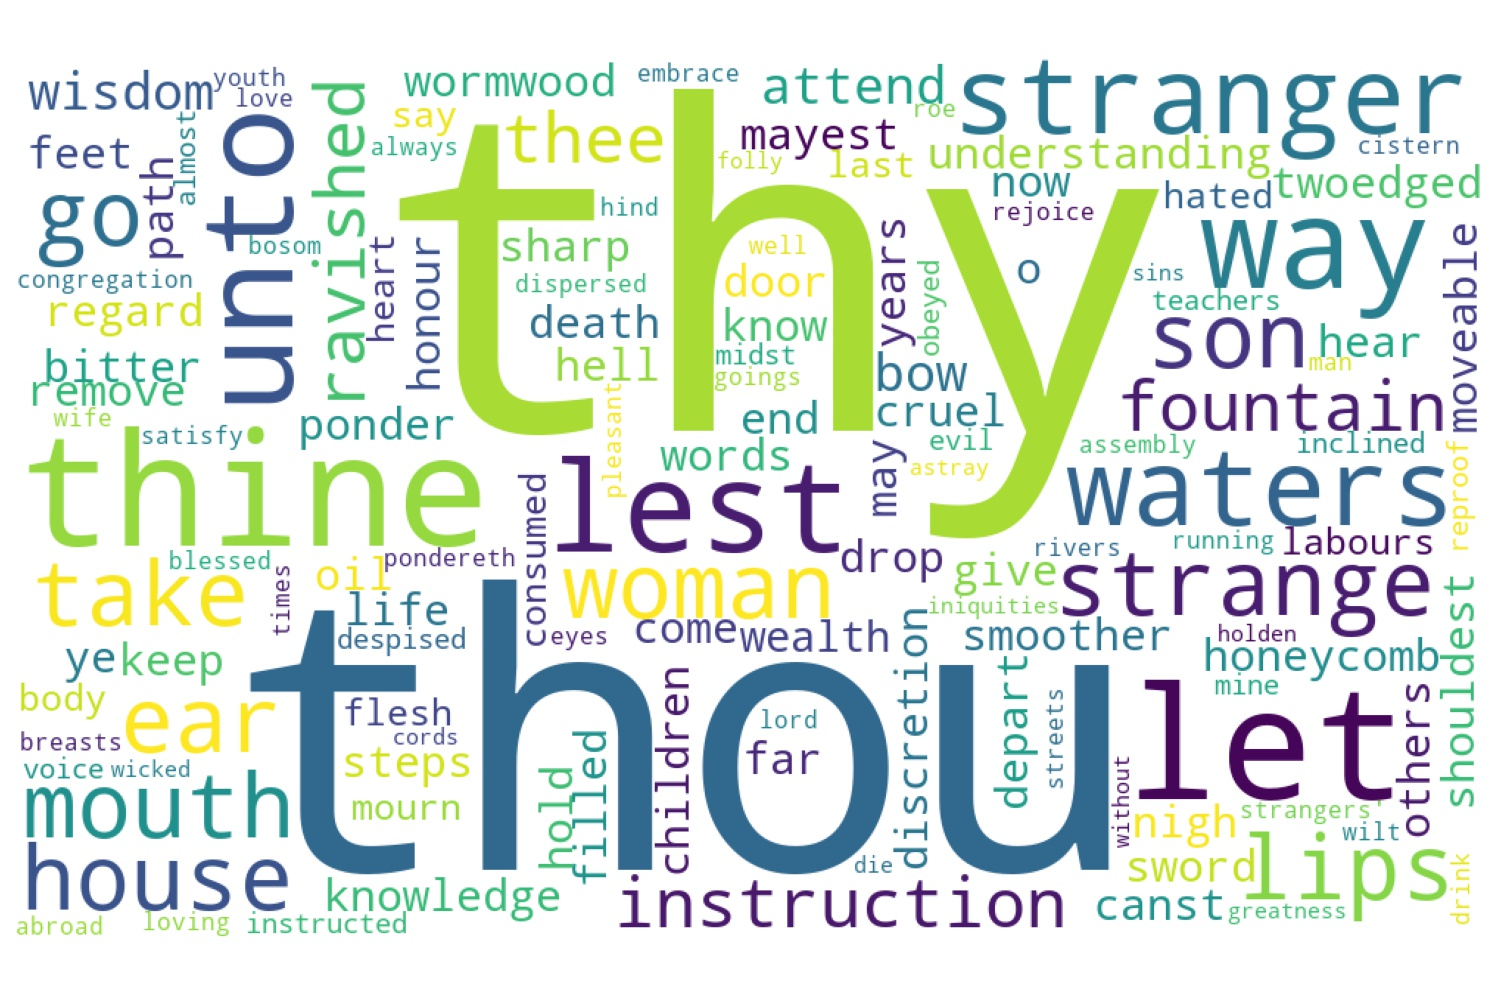
\includegraphics[width=\linewidth]{20OT-Proverbs/Proverb5-WordCloud.jpg}
  \caption{Proverb 5 Word Cloud}
  \label{fig:Proverb 5 Word Cloud}
\end{figure}

\marginpar{\scriptsize \centering \fcolorbox{bone}{lime}{\textbf{REGRETS}}\\ (Proverb 5:3-13) \begin{compactenum}[I.][8]
    \item  \textbf{Chased the Honeycomb!} \index[scripture]{Proverbs!Pro 05:03}(Pro 5:3)
    \item  \textbf{Wasted His Health} \index[scripture]{Proverbs!Pro 05:11}(Pro 5:11)
    \item  \textbf{Gave Away his Honor} \index[scripture]{Proverbs!Pro 05:09}(Pro 5:9)
    \item \textbf{Hated Instruction} \index[scripture]{Proverbs!Pro 05:12}(Pro 5:12)
    \item Did Not \textbf{Heed Correction} \index[scripture]{Proverbs!Pro 05:12}(Pro 5:12)
    \item Did Not \textbf{Harken Unto Teachers} \index[scripture]{Proverbs!Pro 05:13}(Pro 5:13)
    \item Did Not \textbf{Hear His Instructors} \index[scripture]{Proverbs!Pro 05:13}(Pro 5:13)
\end{compactenum}}

\marginpar{\scriptsize \centering \fcolorbox{bone}{yellow}{\textbf{THINE OWN CISTERN}}\\ (Proverb 5:25-21) \begin{compactenum}[I.][8]
    \item \textbf{Running Waters} \index[scripture]{Proverbs!Pro 05:15}(Pro 5:15)
    \item The \textbf{Reserving} \index[scripture]{Proverbs!Pro 05:17}(Pro 5:17)
    \item The \textbf{Rejoicing} \index[scripture]{Proverbs!Pro 05:18}(Pro 5:18)
    \item The \textbf{Roe} \index[scripture]{Proverbs!Pro 05:19}(Pro 5:19)
    \item The \textbf{Ravished} \index[scripture]{Proverbs!Pro 05:19}\index[scripture]{Proverbs!Pro 05:20}(Pro 5:19, 20)
    \item A \textbf{Rejection} \index[scripture]{Proverbs!Pro 05:20}(Pro 5:20)
    \item A \textbf{Review} \index[scripture]{Proverbs!Pro 05:21}(Pro 5:21)
\end{compactenum}}

\marginpar{\scriptsize \centering \fcolorbox{bone}{black}{\textbf{\textcolor[cmyk]{0,0,0,0}{STAY PURE \& ENJOY IT}}}\\ (Proverb 5) 
\begin{compactenum}[I.][8]
    \item The \textbf{Father's Appeal} \index[scripture]{Proverbs!Pro 05:01} \index[scripture]{Proverbs!Pro 05:07} (Pro 5:1, 7)
    \item The \textbf{Fleshly Appetite} 
    \item The \textbf{Fatal Attraction}   \index[scripture]{Proverbs!Pro 05:03-05}  (Pro 5:3-5)
    \item The \textbf{Foolish Absurdity}   \index[scripture]{Proverbs!Pro 05:21}  (Pro 5:21)
    \item The \textbf{Faithful Attention}  
    \item The \textbf{Fruitful Arrangement}   \index[scripture]{Proverbs!Pro 05:15-19}  (Pro 5:15-19)
    \item The \textbf{Final Accountability}   \index[scripture]{Proverbs!Pro 05:21}  (Pro 5:21)
\end{compactenum}}

\marginpar{\scriptsize \centering \fcolorbox{bone}{blue}{\textbf{\textcolor[cmyk]{0,0,0,0}{SEE THE SEDUCTRESS}}}\\ (Proverbs 5) 
\begin{compactenum}[I.][8]
    \item She has lips of honey \index[scripture]{Proverbs!Pro 05:03} (Pro 5:3) 
    \item She has a mouth smooth as oil \index[scripture]{Proverbs!Pro 05:03} (Pro 5:3)
    \item Her end is as bitter wormwood \index[scripture]{Proverbs!Pro 05:04} (Pro  5:4)
    \item Her feet walk the road to ruin \index[scripture]{Proverbs!Pro 05:05} (Pro 5:5)
    \item Her steps (direction) are to death \index[scripture]{Proverbs!Pro 05:05} (Pro 5:5)
\end{compactenum}}

\footnote{\textcolor[cmyk]{0.99998,1,0,0}{\hyperlink{TOC}{Return to end of Table of Contents.}}}\footnote{\href{https://audiobible.com/bible/bible.html}{\textcolor[cmyk]{0.99998,1,0,0}{Proverbs Audio}}}\textcolor[cmyk]{0.99998,1,0,0}{My\textcolor{jungle}{$_{1788}$} son, attend unto my wisdom, \emph{and} bow thine ear to my \fcolorbox{bone}{MYGOLD}{understanding}:}
[2] \textcolor[cmyk]{0.99998,1,0,0}{That\textcolor{jungle}{$_{1801}$} thou mayest regard discretion, and \emph{that} thy lips may keep knowledge.}\\
\\
\P \textcolor[cmyk]{0.99998,1,0,0}{For\textcolor{jungle}{$_{18`3}$} the lips of a strange woman drop \emph{as} an \fcolorbox{bone}{lime}{honeycomb}, and her mouth \emph{is} smoother than oil:}\footnote{\textbf{Hebrews 4:12} - For the word of God is quick, and powerful, and sharper than any twoedged sword, piercing even to the dividing asunder of soul and spirit, and of the joints and marrow, and is a discerner of the thoughts and intents of the heart.}
[4] \textcolor[cmyk]{0.99998,1,0,0}{But\textcolor{jungle}{$_{1831}$} her end is bitter as wormwood, sharp as a twoedged sword.}
[5] \textcolor[cmyk]{0.99998,1,0,0}{Her\textcolor{jungle}{$_{1843}$} feet go down to death; her steps take hold on hell.}
[6] \textcolor[cmyk]{0.99998,1,0,0}{Lest\textcolor{jungle}{$_{1855}$} thou shouldest ponder the path of life, her ways are moveable, \emph{that} thou canst not know \emph{them}.}\footnote{\textbf{Psalm 16:11} - Thou wilt shew me the path of life: in thy presence is fulness of joy; at thy right hand there are pleasures for evermore.}\footnote{\textbf{Psalm 27:11} - Teach me thy way, O LORD, and lead me in a plain path, because of mine enemies.}\footnote{\textbf{Psalm 139:3} - Thou compassest my path and my lying down, and art acquainted with all my ways.}\footnote{\textbf{Psalm 142:3} - When my spirit was overwhelmed within me, then thou knewest my path. In the way wherein I walked have they privily laid a snare for me.}
[7] \textcolor[cmyk]{0.99998,1,0,0}{Hear\textcolor{jungle}{$_{1873}$} me now therefore, O ye children, and depart not from the words of my mouth.}
[8] \textcolor[cmyk]{0.99998,1,0,0}{Remove\textcolor{jungle}{$_{1889}$} thy way far from her, and come not nigh the door of her house:}
[9] \textcolor[cmyk]{0.99998,1,0,0}{Lest\textcolor{jungle}{$_{1904}$} thou give thine honour unto others, and thy years unto the cruel:}
[10] \textcolor[cmyk]{0.99998,1,0,0}{Lest\textcolor{jungle}{$_{1917}$} strangers be filled with thy wealth; and thy labours \emph{be} in the house of a stranger;}
[11] \textcolor[cmyk]{0.99998,1,0,0}{And\textcolor{jungle}{$_{1934}$} thou mourn at the last, when thy \fcolorbox{bone}{lime}{flesh and thy body are consumed},}
[12] \textcolor[cmyk]{0.99998,1,0,0}{And\textcolor{jungle}{$_{1948}$} say, How have I \fcolorbox{bone}{lime}{hated instruction}, and my heart \fcolorbox{bone}{lime}{despised reproof};}
[13] \textcolor[cmyk]{0.99998,1,0,0}{And\textcolor{jungle}{$_{1960}$} have not obeyed \fcolorbox{bone}{lime}{the voice of my teachers}, nor \fcolorbox{bone}{lime}{inclined mine ear} to them that instructed me!}
[14] \textcolor[cmyk]{0.99998,1,0,0}{I\textcolor{jungle}{$_{1978}$} was almost in all evil in the midst of the congregation and assembly.}\\
\\
\P \textcolor[cmyk]{0.99998,1,0,0}{Drink\textcolor{jungle}{$_{1992}$} waters out of thine own cistern, and running waters out of thine own well.}\footnote{\textbf{2 Kings 18:31} - Hearken not to Hezekiah: for thus saith the king of Assyria, Make an agreement with me by a present, and come out to me, and then eat ye every man of his own vine, and every one of his fig tree, and drink ye every one the waters of his cistern:}\footnote{\textbf{Isaiah 36:16} - Hearken not to Hezekiah: for thus saith the king of Assyria, Make an agreement with me by a present, and come out to me: and eat ye every one of his vine, and every one of his fig tree, and drink ye every one the waters of his own cistern;}
[16] \textcolor[cmyk]{0.99998,1,0,0}{Let\textcolor{jungle}{$_{2007}$} thy fountains be dispersed abroad, \emph{and} rivers of waters in the streets.}\footnote{\textbf{Psalm 127:4-5} - As arrows are in the hand of a mighty man; so are children of the youth. [5] Happy is the man that hath his quiver full of them: they shall not be ashamed, but they shall speak with the enemies in the gate.}
[17] \textcolor[cmyk]{0.99998,1,0,0}{Let\textcolor{jungle}{$_{2020}$} them be only thine own, and not strangers' with thee.}
[18] \textcolor[cmyk]{0.99998,1,0,0}{Let\textcolor{jungle}{$_{2031}$} thy fountain be blessed: and rejoice with the wife of thy youth.}
[19] \textcolor[cmyk]{0.99998,1,0,0}{\emph{Let}\textcolor{jungle}{$_{2044}$} \emph{her} \emph{be} \emph{as} the loving hind and pleasant roe; let her breasts satisfy thee at all times; and be thou ravished always with her love.}
[20] \textcolor[cmyk]{0.99998,1,0,0}{And\textcolor{jungle}{$_{2070}$} why wilt thou, my son, be ravished with a strange woman, and embrace the bosom of a stranger?}
[21] \textcolor[cmyk]{0.99998,1,0,0}{For\textcolor{jungle}{$_{2089}$} the ways of man \emph{are} before the eyes of the LORD, and he pondereth all his goings.}\\
\\
\P \textcolor[cmyk]{0.99998,1,0,0}{His\textcolor{jungle}{$_{2107}$} own iniquities shall take the wicked himself, and he shall be holden with the cords of his sins.}
[23] \textcolor[cmyk]{0.99998,1,0,0}{He\textcolor{jungle}{$_{2126}$} shall die without instruction; and in the greatness of his folly he shall go astray\textcolor{jungle}{$_{2141}$}.}




